% Template for FMI-2011 paper; to be used with:
%          fmiconf.sty - LaTeX style file, and
%          IEEEbib.bst - IEEE bibliography style file.
% --------------------------------------------------------------------------
\documentclass{article}
\usepackage{fmiconf,amsmath,epsfig}

\usepackage{german}
\usepackage[utf8]{inputenc}
\usepackage{url}

% Example definitions.
\def\x{{\mathbf x}}
\def\L{{\cal L}}

% Title.
\title{Kann eine Drohne präzise nur mit den Sensoren eines Smartphones gesteuert werden?}
\name{Stefan Baumann, Florian Gümbel}
\address{Technische Hochschule Mittelhessen}

\begin{document}
\maketitle
\begin{abstract}
Drohne ist mittlerweile ein fest etablierter Begriff, der ein von vier Propellern und Elektromotor angetriebenes Flugobjekt beschreibt. Die Steuerung erfolgt zumeist über eine Anwendung auf Smartphone / Tablet. Dabei wird hauptsächlich ein virtueller Joystick auf dem Bildschirm angezeigt der mit Gesten gesteuert wird.\\ Eine andere aber bisher aber weitestgehend eingeschränkt genutzte Art der Steuerung ist der Einsatz von Hilfe Gyro- und Bewegungssensor des Smartphones. Eingeschränkt insofern, als dass nicht alle Möglichkeiten der Sensoren genutzt werden. An diesem Ansatz soll mit der Entwicklung einer nativen Android App für Smartphones angeknüpft werden. Ziel ist es, die Bewegungen, die vom Benutzer mit dem Smartphone getätigt werden, an die Drohne zu übertragen. Zusätzlich sollen Gesten das Steuern von Foto- und Vieoaufnahmen und deren Übertragung auf das Display des Smartphones vervollständigen.\\ Am Ende gilt es die Frage zu beantworten, ob die Steuerung einer Drohne präzise genug ist, wenn diese komplett auf Gyroskop und Accelerometer des Smartphones gekoppelt ist.

\end{abstract}

\section{Einleitung}
\label{sec:einleitung}
Immer mehr erfreuen sich sogenannte Drohnen an Beliebtheit. Diese neue Form des unbemannten Flugobjekte zeichnet sich zumeist dadurch aus, dass sie, anders als herkömmliche bekannte Modellflugzeuge, mindestens vier kleine Propeller hat welche über Elektromotoren angetrieben werden und die Drohne senkrecht starten lassen. Die Anzahl der Propeller kann variieren. Angefangen von Quadrocopter über Hexacopter und Octacopter bis hin zu Multicopter. Der Einsatzzweck einer solchen Drohne geht von Vermessungstechnik über Luftaufnahmen und Erkundung bis hin zur Jagd.

Um eine Solche Drohne zu Steuern gibt es verschiedene Möglichkeiten. Abhängig von Modell lassen sich klassische Fernsteuerungen entweder direkt mit der Drohne Verbinden oder über Umweg mit Hilfe einer App. Nahezu jeder Drohnenhersteller bietet eine eigene App für alle gängigen Smartphones oder Tablets an. Die Verbindung findet je nach Modell über W-Lan oder Bluetooth statt. Für die Steuerung mittels App auf dem Gerät steht ein digitaler Joystick zur Verfügung dessen Bewegung umgerechnet und auf die Drohne Übertragen wird während das Gerät ruhig in der Hand liegt. Meistens wird über den linken Joystick die vertikale Bewegung gesteuert. Dazu zählt die Veränderung Höhe und die Drehung in beide Richtungen. Der Rechte Joystick ist für die horizontale Bewegung zuständig. Damit ist das Schwenken zur Seite sowie das Vorwärts- und Rückwärtsfliegen gemeint. Teilweise werden auch Sensoren zu Steuerung unterstützt.
\\ Die Idee ist es nun, eine weitere Möglichkeit zu untersuchen, bei der zwei Sensoren des Smartphones für die gesamte Steuerung zum Einsatz kommen. Dabei soll anstelle der Bedienung auf dem Touchscreen nur das Gerät als Steuerungseinheit genutzt werden. \\Gyroskop und Accelerometer dienen zur Erfassung der Bewegungen worauf das Smartphone diese auf die Drohne übeträgt. 
\begin{figure}[htb]
\begin{minipage}[b]{1.0\linewidth}
  \centering
\centerline{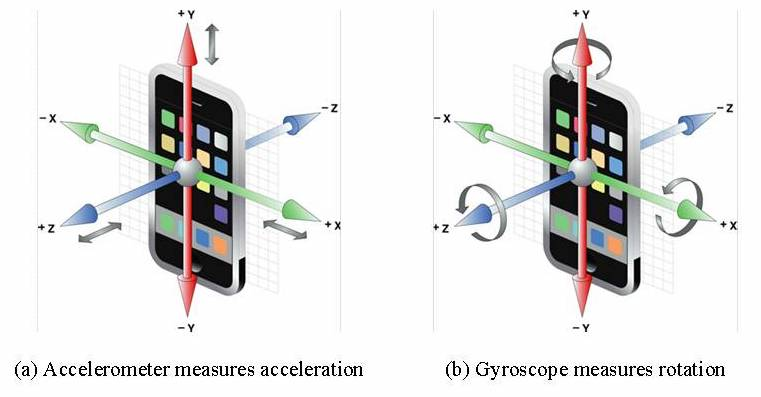
\includegraphics[width= 85mm]{gyro.jpg}}
\end{minipage}
\caption{Accelerometer und Gyroscope (Quelle: Apple Inc.)}
\label{fig:gyro}
\end{figure}


\section{Stand der Technik}
\label{sec:verwandteArbeiten}
\subsection{Drohnensteuerung}
Neben vielen Drittherstelleranwendungen bieten, wie bereits in der Einleitung erwähnt, auch die Hersteller der Drohnen eigene Anwendungen zum steuern der Drohne an.
\\ Die bekannte Firma Parrot stellt eine Vielzahl verschiedener Apps zum Steuern bereit. Eine davon ist die FreeFlight-App \footnote{https://play.google.com/store/apps/details?id=com.parrot.freeflight\&hl=de}, die Steuerung durch den Gyroscope-Sensor unterstützt. Dabei fliegt die Drohne in die Richtung in der das Smartphone geneigt wird ohne sich dabei nach vorne zu drehen. Eine Höhenveränderung oder Drehen ist nicht möglich. Auf eine Implementierung des Accelerometer wurde hierbei verzichtet.
\\Bereits Anfang 2015 hat Sony ein Projekt vorgestellt, in dem eine Drohne mittels SmartWatch 2, SmartEyeglass und Smartphone gesteuert wird \footnote{http://developer.sonymobile.com/2015/01/05/control-a-mini-drone-with-smarteyeglass-and-smartwatch-2-tutorial/}. In diesem Fall ist die SmartWatch via Bluetooth mit dem Smartphone verbunden und überträgt die Bewegung per W-Lan an die Drohne. Über das Display der Smartwatch lassen sich dabei die verschiedenen Steuerungs-Modi umschalten. Hier kommen sowohl Accelerometer als auch Gyroscope zum Einsatz.

\subsection{Einsatz von Sensoren}
Die Sensoren finden in vielen Bereichen Verwendung und sind bereits in jedem aktuellen Smartphone Standard. Sie werden meistens in Kombination genutzt wie beispielsweise bei der Erkennung von Bewegungsänderung oder der Messung von physischen Aktivitäten \cite{wu2012classification}. 
\\Um die derzeitige Lage oder Beschleunigung des Gerätes zu ermitteln, kommt der Accelerometer oder auch Beschleunigungssensor zum Einsatz. Mittels der Schwerkraft wird ermittelt in welche Richtung das Smartphone bewegt wird. In der Regel kommen die X- Y- und Z-Achse zum Einsatz. Die rotatorische Geschwindigkeit und somit auch die Drehbewegung des Smartphones werden vom Gyroskop gemessen. Dazu wird die Corioliskraft und das sogenannte Stimmgabelprinzip genutzt. Hier kommen Längs- Quer und Hochachse für die Positionsbestimmung im Raum zum Einsatz.

\section{Methodik}

\subsection{Eingesetzte Drohne und verwendete Technologien}
Als Testdrohne wurde für eine Parrot Airborne Night Drone der Kategorie Mini-Drohne entschieden\footnote{https://www.parrot.com/de/minidrohnen/parrot-airborne-night-maclane#parrot-airborne-night-maclane}, da sie folgende Vorteile mit sich bringt: 
\begin{itemize}
	\item Relativ geringen Anschaffungspreis
	\item Unterstützt das aktuelle Parrot SDK3
	\item Gute Testbarkeit in Gebäuden durch geringe Größe 
\end{itemize}

Wie in den vorangegangenen Kapitel schon erläutert wurde, gibt es aktuell keine App die eine volle Steuerung über die Sensoren unterstützt. Aus diesen Gründen wurde zu Testzwecken ein Prototyp entwickelt, welcher die gestellten Anforderungen erfüllt.Aus Gründen der Flexibilität wurde für die Umsetzung des Prototypen für eine native Android-Anwendung entschieden.\\ Als Verbindung zwischen Anwendung und Drohne kommt Bluetooth zum Einsatz. 

\subsection{}

\section{Ergebnisse und Evaluation}


\section{Zusammenfassung und Ausblick}
\bibliography{Template}{}
\bibliographystyle{IEEEbib}
\end{document}